\documentclass[aspectratio=169]{beamer}

% ── Theme ────────────────────────────────────────────────────────────────────
\usetheme{Madrid}
\usecolortheme{default}
\setbeamertemplate{navigation symbols}{}

% ── Packages ─────────────────────────────────────────────────────────────────
\usepackage{booktabs}
\usepackage{microtype}
\usepackage{xcolor}
\usepackage{listings}
\usepackage{tikz}
\usetikzlibrary{arrows.meta, positioning, shapes.geometric, fit, backgrounds, calc}
\usepackage{fontawesome5}
\usepackage{multirow}
\usepackage{array}
\usepackage{amsmath}
\usepackage{graphicx}

% ── Footline: X / N where N = main-slide count ──────────────────────────────
\newcounter{mainframes}

\makeatletter
\newcommand{\savemainframecount}{%
  \immediate\write\@auxout{%
    \string\setcounter{mainframes}{\the\c@framenumber}%
  }%
}
\makeatother

\setbeamertemplate{footline}{%
  \hfill{\color{gray}\scriptsize
    \ifnum\value{mainframes}>0
      \insertframenumber\,/\,\themainframes
    \else
      \insertframenumber
    \fi
  }\hspace*{2ex}\vskip4pt%
}

% ── Colours ──────────────────────────────────────────────────────────────────
\definecolor{symptom}    {HTML}{E57373}   % red
\definecolor{condition}  {HTML}{64B5F6}   % blue
\definecolor{testcol}    {HTML}{81C784}   % green
\definecolor{vital}      {HTML}{FFB74D}   % orange
\definecolor{demo}       {HTML}{CE93D8}   % purple
\definecolor{riskfactor} {HTML}{FFF176}   % yellow
\definecolor{moi}        {HTML}{F48FB1}   % rose
\definecolor{attribute}  {HTML}{80CBC4}   % mint
\definecolor{treatment}  {HTML}{A5D6A7}   % light green
\definecolor{adverseev}  {HTML}{FFCCBC}   % peach

\definecolor{darkblue}   {HTML}{1A237E}
\definecolor{midblue}    {HTML}{1565C0}
\definecolor{lightgray}  {HTML}{F5F5F5}

\setbeamercolor{frametitle}      {bg=darkblue, fg=white}
\setbeamercolor{title}           {fg=white}
\setbeamercolor{palette primary} {bg=darkblue, fg=white}
\setbeamercolor{palette secondary}{bg=midblue,  fg=white}
\setbeamercolor{structure}       {fg=darkblue}

% ── Listing style ─────────────────────────────────────────────────────────────
\lstset{
  basicstyle=\ttfamily\footnotesize,
  backgroundcolor=\color{lightgray},
  frame=single,
  rulecolor=\color{gray!40},
  breaklines=true,
  columns=fullflexible,
  keepspaces=true,
}

% ── Helper commands ───────────────────────────────────────────────────────────
\newcommand{\nodebox}[2]{%
  \colorbox{#1}{\strut\small\textbf{#2}}%
}

% ── Metadata ─────────────────────────────────────────────────────────────────
\title[MLMD Noise]{Reading between the lines}
\subtitle{LLM-based label imputation and meta-learning\\for noisy labels in emergency department triage}
\author{Alice Chua \and Tyler Biswurm}
\institute{%
  LMP2392H --- Healthcare and Medicine for AI Experts\\[0.3em]
  \small Supervisor: Anna Goldenberg \quad Co-supervisor: Ismail Akrout
}
\date{Progress report --- \today}

% ─────────────────────────────────────────────────────────────────────────────
\begin{document}
% ─────────────────────────────────────────────────────────────────────────────

% ── Title slide ───────────────────────────────────────────────────────────────
\begin{frame}
  \titlepage
\end{frame}

% ── Outline ───────────────────────────────────────────────────────────────────
\begin{frame}{Outline}
  \tableofcontents
\end{frame}

% =============================================================================
\section{Clinical motivation}
% =============================================================================

\begin{frame}{Problem: noisy labels in emergency triage}
  \begin{columns}[T]
    \begin{column}{0.52\textwidth}
      \textbf{SickKids MLMD system}
      \begin{itemize}
        \item Authorizes diagnostics at triage --- before the physician ---
              parallelizing test processing with queue time.
        \item Silent trial complete; clinical trial next.
        \item Bottleneck: \textbf{label noise} suppresses recall.
      \end{itemize}
      \vspace{0.8em}
      \textbf{Root cause}
      \begin{itemize}
        \item EHR misses externally-performed tests.
        \item False negatives look identical to true negatives.
        \item Model learns spurious absences\\
              (e.g.,\ chest pain $\not\Rightarrow$ ECG).
      \end{itemize}
    \end{column}
    \begin{column}{0.44\textwidth}
      \begin{block}{MLMD deployment}
        \small
        \faCheck\; Silent trial complete\\
        \faArrowRight\; Clinical trial pending
      \end{block}

      \vspace{0.5em}
      \begin{block}{Five test pathways in scope}
        \small
        \begin{itemize}
          \item[\faHeartbeat]    ECG
          \item[\faSearch]       Testicular ultrasound
          \item[\faBone]         Arm X-ray
          \item[\faNotesMedical] Abdominal ultrasound
          \item[\faNotesMedical] Appendix area ultrasound
        \end{itemize}
      \end{block}
    \end{column}
  \end{columns}
\end{frame}

% =============================================================================
\section{Data and setting}
% =============================================================================

\begin{frame}{The SickKids dataset}
  \begin{columns}[T]
    \begin{column}{0.52\textwidth}
      \textbf{Dataset}
      \begin{itemize}
        \item \textbf{520\,000} ED visits --- SickKids EHR.
        \item Triage-time features: vitals, CTAS score,
              chief complaint, demographics.
        \item Labels: 5 binary test-ordered flags.
      \end{itemize}
      \vspace{0.5em}
      \textbf{Asymmetric noise}
      \begin{itemize}
        \item Positives: reliable ground truth.
        \item Negatives: true negatives \emph{or}
              unobserved external tests.
      \end{itemize}
    \end{column}
    \begin{column}{0.44\textwidth}
      \begin{block}{Diagnosis field (\texttt{dx})}
        \small
        Free-text column with semicolon-separated diagnoses
        (manual clinician input, post-assessment).\\[0.3em]
        Our label imputation pipeline extracts this field
        to build the diagnosis$\to$test mapping.
      \end{block}

      \vspace{0.4em}
      \begin{block}{High transfer rate}
        \small
        SickKids receives many transfers from community
        hospitals; tests performed at referring sites
        are the primary source of false-negative labels.
      \end{block}
    \end{column}
  \end{columns}
\end{frame}

% =============================================================================
\section{Relevant work}
% =============================================================================

\begin{frame}{Relevant work}
  \begin{columns}[T]
    \begin{column}{0.48\textwidth}
      \textbf{LLMs + knowledge graphs}
      \begin{itemize}\footnotesize
        \item \textbf{Yao et al.\ (2025):} LLMs imputing
              disease$\to$treatment edges in medical KGs show
              low recall and hallucinations, motivating
              KG-grounded evaluation.
        \item \textbf{Li et al.\ (2025):} Knowledge-conditioned LLMs
              improve accuracy of clinical data extraction.
        \item \textbf{Cao et al.\ (2026):} LLM-powered knowledge
              graphs enable real-time clinical analytics at scale
              (JAMIA Open).
        \item \textbf{Han et al.\ (2026):} Denoise2Impute ---
              distinguishes true negatives from unknown-missing
              positives to recover missing diagnosis codes in EHRs.
      \end{itemize}
    \end{column}
    \begin{column}{0.48\textwidth}
      \textbf{Noise-robust training}
      \begin{itemize}\footnotesize
        \item \textbf{Yang et al.\ (2024):} CV-style label noise
              techniques (label smoothing, MixUp, NCR) improve EHR
              classifiers under asymmetric false-positive/negative rates.
        \item \textbf{Ren et al.\ (2018):} Meta-learning to reweight
              training examples; foundational approach for noisy labels.
        \item \textbf{Northcutt et al.\ (2021):} Confident Learning ---
              characterising and filtering label errors using predicted
              probabilities.
        \item \textbf{Moturu et al.\ (2025):} LiLAW --- 3 learnable
              parameters adapt per-sample weights via bilevel optimisation.
      \end{itemize}
    \end{column}
  \end{columns}
\end{frame}

% =============================================================================
\section{Approach}
% =============================================================================

\begin{frame}{Two complementary strategies}
  \centering
  \vspace{0.5em}
  \begin{columns}[c]
    \begin{column}{0.44\textwidth}
      \begin{block}{\centering Label imputation}
        \small
        \textbf{Goal:} clean the training data.\\[0.3em]
        Build a knowledge graph from clinical guidelines;
        use it to identify and correct false negatives
        in the EHR labels.\\[0.3em]
        \textit{Fixes deterministic cases}\\
        (diagnosis clearly implies test).
      \end{block}
    \end{column}
    \begin{column}{0.44\textwidth}
      \begin{block}{\centering Robust training}
        \small
        \textbf{Goal:} train robustly on residual noise.\\[0.3em]
        Meta-learn per-sample loss weights that
        down-weight suspected false negatives
        during training.\\[0.3em]
        \textit{Handles probabilistic cases}\\
        (chest pain \emph{sometimes} warrants ECG).
      \end{block}
    \end{column}
  \end{columns}
\end{frame}

% =============================================================================
\section{Label imputation}
% =============================================================================

\begin{frame}{Label imputation: end-to-end pipeline}
  \centering
  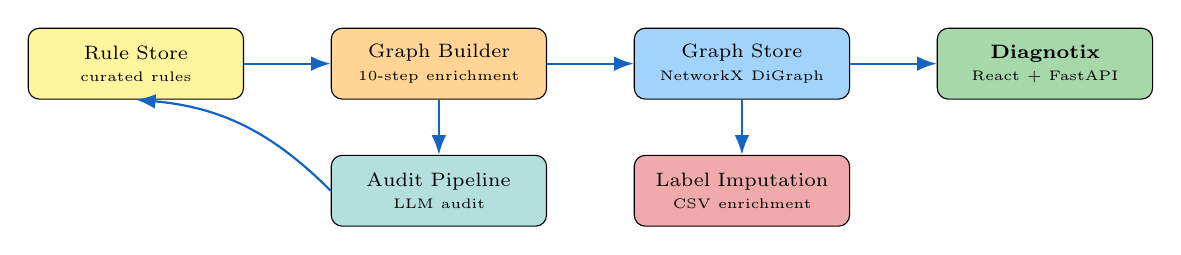
\begin{tikzpicture}[
    node distance=0.7cm and 1.1cm,
    box/.style={draw, rounded corners, fill=lightgray,
                text width=2.5cm, align=center, minimum height=0.9cm,
                font=\scriptsize},
    arr/.style={-{Latex[length=2.5mm]}, thick, color=midblue},
  ]
    \node[box, fill=riskfactor!70] (json)
      {Rule Store\\{\tiny curated rules}};

    \node[box, fill=vital!60, right=of json] (build)
      {Graph Builder\\{\tiny 10-step enrichment}};

    \node[box, fill=condition!60, right=of build] (pkl)
      {Graph Store\\{\tiny NetworkX DiGraph}};

    \node[box, fill=testcol!70, right=of pkl] (diagnotix)
      {\textbf{Diagnotix}\\{\tiny React + FastAPI}};

    \node[box, fill=symptom!60, below=of pkl] (pipe)
      {Label Imputation\\{\tiny CSV enrichment}};

    \node[box, fill=attribute!60, below=of build] (audit)
      {Audit Pipeline\\{\tiny LLM audit}};

    \draw[arr] (json)         -- (build);
    \draw[arr] (build)        -- (pkl);
    \draw[arr] (pkl)          -- (diagnotix);
    \draw[arr] (pkl)          -- (pipe);
    \draw[arr] (build.south)  -- (audit.north);
    \draw[arr] (audit.west)   to[bend right=20] (json.south);
  \end{tikzpicture}

  \vspace{0.4em}
  \small
  \begin{enumerate}
    \item Rules iteratively audited and revised until satisfactory.
    \item Graph builder serialises the enriched graph.
    \item Graph store powers label imputation and the \textbf{Diagnotix} web app.
  \end{enumerate}
\end{frame}

\begin{frame}[fragile]{Label imputation: from rules to enriched graph}
  \begin{columns}[T]
    \begin{column}{0.47\textwidth}
      \vspace{0.2em}
      \begin{center}
        \texttt{symptom} \;$\longrightarrow$\; \texttt{condition} \;$\longrightarrow$\; \texttt{test}
      \end{center}

      \vspace{0.3em}
      \begin{exampleblock}{Example rule (JSON)}
        \begin{lstlisting}[language={}]
{
  "raw_symptom": "chest pain",
  "node_type": "Symptom",
  "condition": "Acute MI",
  "test": "ECG",
  "source": "AHA/ACC"
}
        \end{lstlisting}
      \end{exampleblock}
    \end{column}
    \hfill
    \begin{column}{0.49\textwidth}
      \vspace{0.2em}
      \textbf{Enrichment pipeline}\\[0.4em]
      \scriptsize
      \begin{tabular}{@{}cll@{}}
        \toprule
        \textbf{Step} & \textbf{Source} & \textbf{Adds} \\
        \midrule
        \multicolumn{3}{@{}l}{\textit{Foundation}} \\
        0 & LLM rule generation     & base rule set \\
        1 & Curated URL registry    & guideline URLs per test \\
        \midrule
        \multicolumn{3}{@{}l}{\textit{Standardised medical codes}} \\
        2 & EMBL-EBI OLS4           & HP / MONDO codes \\
        3 & Infoway FHIR            & SNOMED CT CA \\
        4 & UMLS REST               & LOINC codes \\
        5--6 & UMLS / Infoway       & ICD-10, ICD-10-CA \\
        \midrule
        \multicolumn{3}{@{}l}{\textit{Evidence signals}} \\
        8--9 & Europe PMC           & literature co-occurrence \\
        10 & ClinicalTrials.gov     & clinical trial counts \\
        \bottomrule
      \end{tabular}
    \end{column}
  \end{columns}
\end{frame}

\begin{frame}{Label imputation: validating LLM-generated rules}
  Our audit pipeline cleans LLM-generated rules before the graph is built.

  \vspace{0.3em}
  \centering
  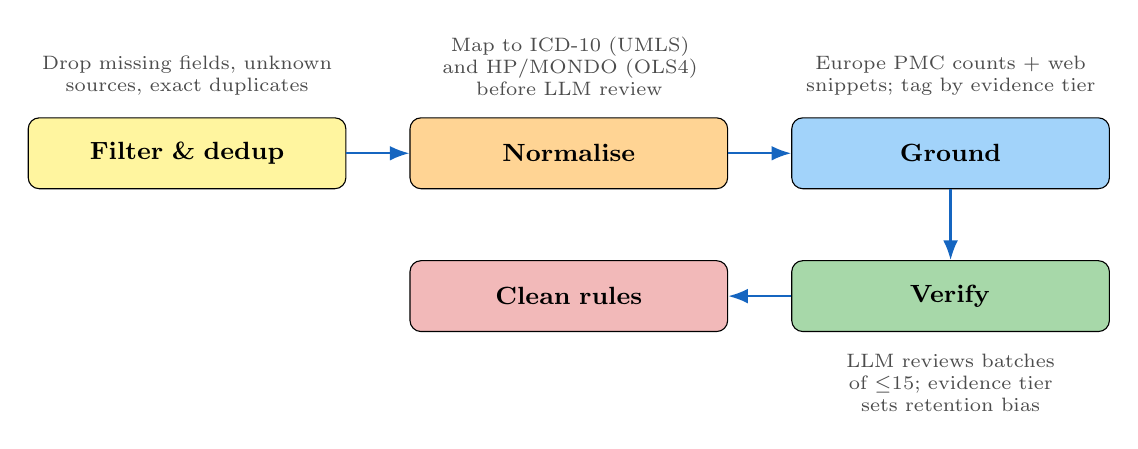
\begin{tikzpicture}[
    node distance=0.5cm and 0.8cm,
    box/.style={draw, rounded corners, fill=lightgray,
                text width=3.8cm, align=center, minimum height=0.9cm,
                font=\small},
    annot/.style={font=\scriptsize, text width=3.8cm, align=center,
                  text=black!70},
    arr/.style={-{Latex[length=2.5mm]}, thick, color=midblue},
  ]
    % Row 1 (left-to-right), captions above
    \node[box, fill=riskfactor!70] (pre)
      {\textbf{Filter \& dedup}};
    \node[box, fill=vital!60, right=of pre] (norm)
      {\textbf{Normalise}};
    \node[box, fill=condition!60, right=of norm] (ground)
      {\textbf{Ground}};

    \node[annot, above=0.15cm of pre]
      {Drop missing fields, unknown sources, exact duplicates};
    \node[annot, above=0.15cm of norm]
      {Map to ICD-10 (UMLS) and HP/MONDO (OLS4) before LLM review};
    \node[annot, above=0.15cm of ground]
      {Europe PMC counts + web snippets; tag by evidence tier};

    % Row 2 (right-to-left), captions below
    \node[box, fill=testcol!70, below=0.9cm of ground] (verify)
      {\textbf{Verify}};
    \node[box, fill=symptom!50, left=of verify] (out)
      {\textbf{Clean rules}};

    \node[annot, below=0.15cm of verify]
      {LLM reviews batches of $\leq$15; evidence tier sets retention bias};

    \draw[arr] (pre)    -- (norm);
    \draw[arr] (norm)   -- (ground);
    \draw[arr] (ground) -- (verify);
    \draw[arr] (verify) -- (out);
  \end{tikzpicture}
\end{frame}

\begin{frame}{Label imputation: Diagnotix web application}
  \centering
  \small Enter any diagnostic test; the system generates and audits
  evidence-based triage rules and adds them to the knowledge graph.\\[0.6em]
  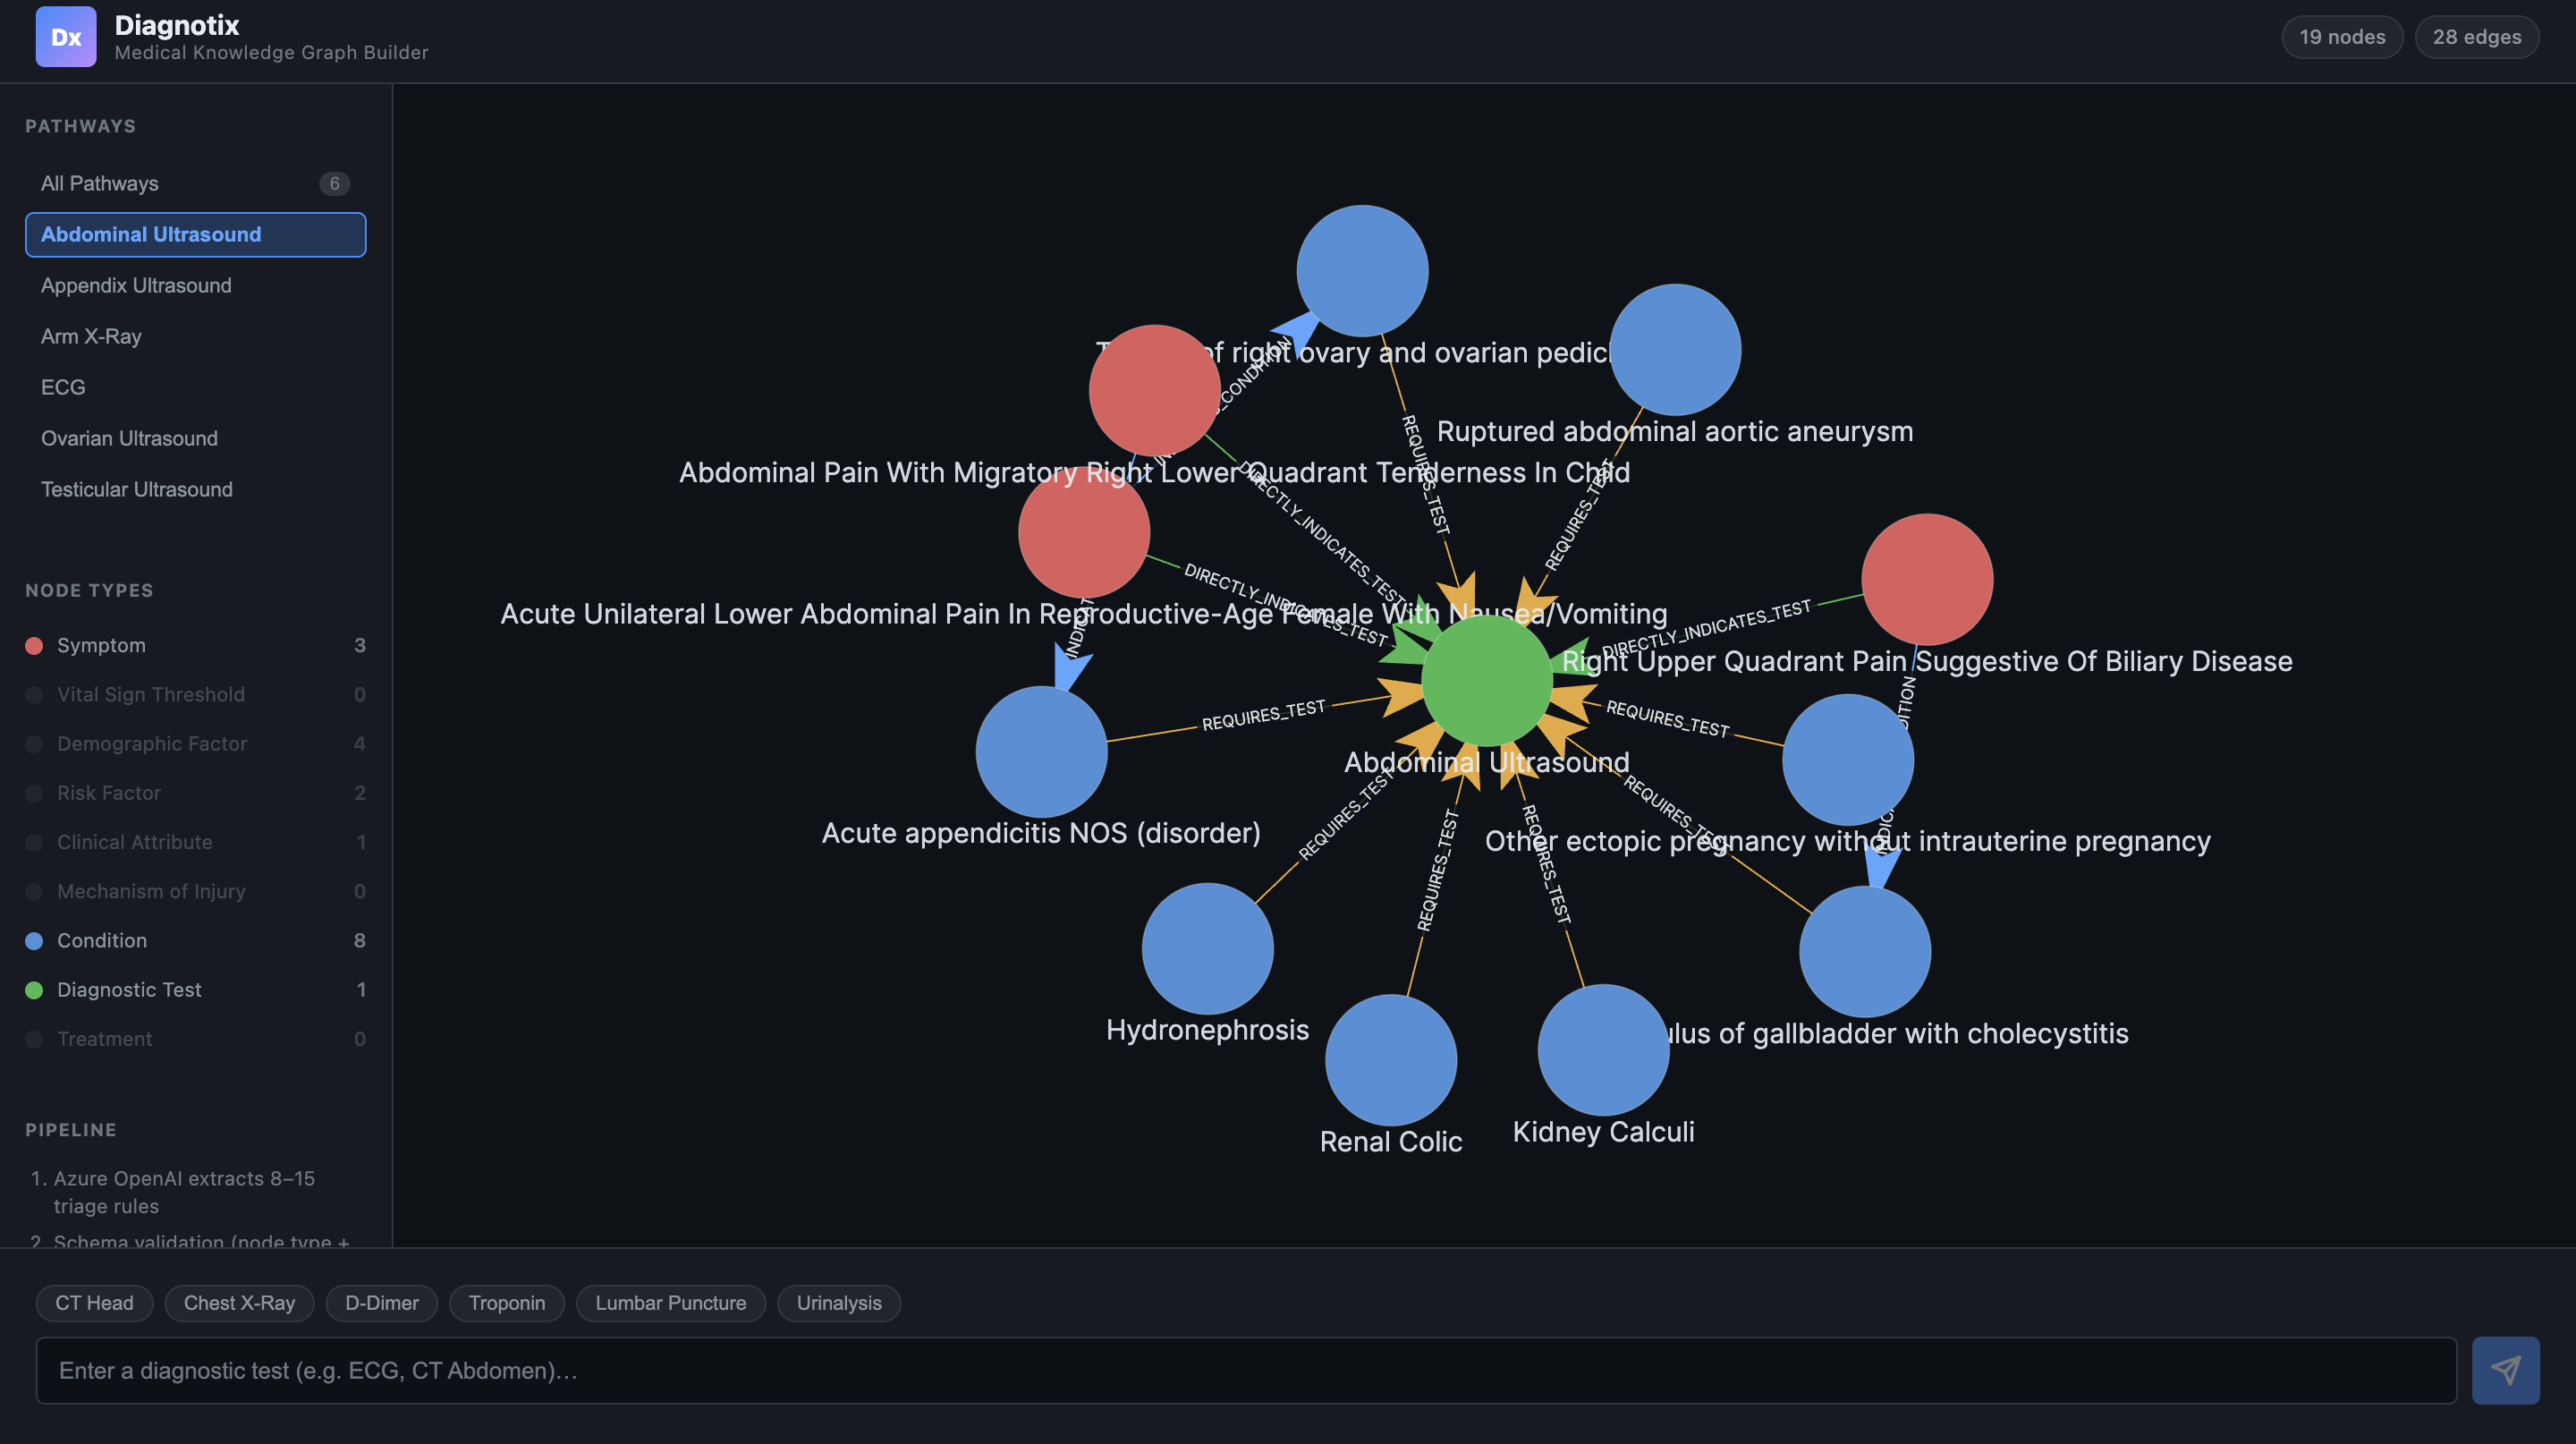
\includegraphics[width=0.75\linewidth]{images/webapp-ss.png}
\end{frame}

% =============================================================================
\section{Robust training}
% =============================================================================

\begin{frame}{Robust training: learning to down-weight noise}
  \begin{columns}[T]
    \begin{column}{0.52\textwidth}
      \textbf{Core idea}
      \begin{itemize}
        \item Learn to \textbf{down-weight} suspected false negatives
              during training --- no manual noise annotations needed.
        \item Three scalar parameters ($\alpha, \beta, \delta$) control
              weighting of easy, moderate, and hard samples.
      \end{itemize}

      \vspace{0.6em}
      \textbf{Mechanism}
      \begin{itemize}
        \item Per-sample weight derived from model confidence:\\
              $\mathcal{W} = \mathcal{W}_\alpha + \mathcal{W}_\beta + \mathcal{W}_\delta$
        \item Bilevel optimisation: model params update on
              weighted training batches; $\alpha, \beta, \delta$ update
              on a validation mini-batch.
      \end{itemize}
    \end{column}
    \begin{column}{0.44\textwidth}
      \begin{block}{Why LiLAW here?}
        \small
        Label imputation fixes \emph{deterministic} false negatives
        (diagnosis clearly implies test).\\[0.4em]
        LiLAW handles \emph{probabilistic} cases
        (chest pain \emph{sometimes} warrants ECG).
      \end{block}

      \vspace{0.5em}
      \begin{block}{Properties}
        \small
        \begin{itemize}
          \item Only 3 extra parameters
          \item 1 extra fwd/bwd pass per batch
          \item No specially curated clean validation set required
        \end{itemize}
      \end{block}
    \end{column}
  \end{columns}
\end{frame}

% =============================================================================
\section{Evaluation plan}
% =============================================================================

\begin{frame}{Evaluation plan}
  \begin{columns}[T]
    \begin{column}{0.48\textwidth}
      \textbf{Four model conditions}
      \begin{enumerate}
        \item Production MLMD baseline
        \item Imputed labels only
        \item LiLAW training only
        \item Imputed labels + LiLAW
      \end{enumerate}

      \vspace{0.6em}
      \textbf{Metrics}
      \begin{itemize}
        \item \textbf{Recall} --- clinical efficiency\\
              {\small (tests authorized $\Rightarrow$ parallel workflow)}
        \item \textbf{Precision} --- patient safety\\
              {\small (unnecessary tests avoided)}
        \item PR curves at multiple operating points
        \item Expected Calibration Error (ECE)
      \end{itemize}
    \end{column}
    \begin{column}{0.48\textwidth}
      \textbf{Additional validation of label imputation}

      \vspace{0.3em}
      \begin{block}{Label recovery benchmark}
        \small
        Mask known positives in held-out data;
        measure knowledge graph's
        ability to recover them.
      \end{block}

      \vspace{0.3em}
      \begin{block}{Future: clinical validation}
        \small
        Clinician review of imputed labels and
        blinded evaluation of retrained model outputs
        during eventual silent / clinical trial.
      \end{block}
    \end{column}
  \end{columns}
\end{frame}

% =============================================================================
\section{Progress and roadmap}
% =============================================================================

\begin{frame}{Progress and roadmap}
  \begin{columns}[T]
    \begin{column}{0.48\textwidth}
      \textbf{Completed}
      \begin{itemize}
        \item[\faCheckSquare] KG rule store: 45 rules, 5 pathways
        \item[\faCheckSquare] 10-step ontology enrichment pipeline
        \item[\faCheckSquare] Evidence-grounded audit pipeline
        \item[\faCheckSquare] Diagnotix web application
      \end{itemize}
    \end{column}
    \begin{column}{0.48\textwidth}
      \textbf{Remaining}
      \begin{enumerate}
        \item Complete label imputation pipeline\\
              {\small (dx $\to$ KG $\to$ recovered labels)}
        \item Implement LiLAW training recipe
        \item Retrain MLMD under 4 conditions
        \item Run evaluation (recall, precision, ECE)
        \item Final delivery of outputs --- \textbf{April 14}
      \end{enumerate}
    \end{column}
  \end{columns}
\end{frame}

% ── Thank you ────────────────────────────────────────────────────────────────

\begin{frame}{}
  \centering
  \vspace{2em}
  {\Large\textbf{Thank you}}

  \vspace{1.5em}
  \begin{columns}[c]
    \begin{column}{0.6\textwidth}
      \small
      \textbf{Happy to discuss:}
      \begin{itemize}
        \item Limitations
        \item KG auditing pipeline
        \item Knowledge graph deep-dive
        \item Diagnotix demo
      \end{itemize}
    \end{column}
  \end{columns}
\end{frame}

% =============================================================================
% APPENDIX
% =============================================================================
\savemainframecount
\appendix

% ── Blank separator ──────────────────────────────────────────────────────────
\begin{frame}{}
\end{frame}

% ── Limitations ──────────────────────────────────────────────────────────────
\begin{frame}{Limitations}
  \begin{columns}[T]
    \begin{column}{0.48\textwidth}
      \textbf{Label imputation}
      \begin{itemize}
        \item LLM-generated diagnosis--test maps may
              hallucinate links (audit pipeline mitigates).
        \item Free-text \texttt{dx} field is noisy and
              inconsistently formatted.
      \end{itemize}
    \end{column}
    \begin{column}{0.48\textwidth}
      \textbf{Training and deployment}
      \begin{itemize}
        \item LiLAW is unproven on real-world clinical
              data with asymmetric label noise.
        \item Data shift: changing referral patterns can
              alter the noise distribution over time.
        \item On-premise access limits experiment
              throughput.
      \end{itemize}
    \end{column}
  \end{columns}

  \vspace{0.8em}
  \textbf{Future validation:} clinician review of imputed labels and
  blinded review of retrained model outputs during eventual
  silent trial / clinical trial of the retrained system.
\end{frame}

% ── Audit detail ─────────────────────────────────────────────────────────────
\begin{frame}{Audit pipeline: evidence grounding and LLM verification (passes 2--3)}
  \begin{columns}[T]
    \begin{column}{0.48\textwidth}
      \begin{block}{Pass 2 --- Evidence grounding}
        \small
        Two signals fetched per rule:
        \begin{itemize}
          \item \textbf{Europe PMC} co-occurrence count
          \item \textbf{DuckDuckGo} web snippets
        \end{itemize}
        \vspace{0.2em}
        Rules tagged by \textbf{PMC evidence tier}:
        \begin{center}
          \footnotesize
          \begin{tabular}{@{}ll@{}}
            \textbf{STRONG}   & $\geq$5\,000 articles \\
            \textbf{GOOD}     & $\geq$500 \\
            \textbf{MODERATE} & $\geq$50 \\
            \textbf{LIMITED}  & $>$0 \\
            \textbf{NONE}     & 0 \\
          \end{tabular}
        \end{center}
      \end{block}
    \end{column}
    \begin{column}{0.48\textwidth}
      \begin{block}{Pass 3 --- LLM clinical verification}
        \small
        LLM reviewer grouped by pathway, batched at \textbf{$\leq$15 rules/call}.

        \vspace{0.2em}
        Evidence tier drives retention bias:
        \begin{itemize}
          \item STRONG / GOOD $\to$ retain by default
          \item MODERATE / LIMITED $\to$ normal scrutiny
          \item NONE $\to$ bias to remove
        \end{itemize}

        \vspace{0.2em}
        Three verification criteria:
        \begin{enumerate}
          \item Source accuracy
          \item Clinical plausibility
          \item Condition specificity
        \end{enumerate}
      \end{block}
    \end{column}
  \end{columns}
\end{frame}

% ── Full graph schema ────────────────────────────────────────────────────────
\begin{frame}{Knowledge graph schema}
  \begin{columns}[T]
    \begin{column}{0.44\textwidth}
      \textbf{Primary node types}\\[0.4em]
      \begin{tabular}{@{}ll@{}}
        \nodebox{symptom!80}{Symptom}     & \texttt{Symptom:} \\[2pt]
        \nodebox{condition!80}{Condition} & \texttt{Condition:} \\[2pt]
        \nodebox{testcol!80}{Test}        & \texttt{Test:} \\
      \end{tabular}

      \vspace{0.6em}
      \textbf{Secondary node types}\\[0.4em]
      \begin{tabular}{@{}ll@{}}
        \nodebox{vital!80}{Vital}            & \texttt{Vital:} \\[2pt]
        \nodebox{demo!70}{Demographic}       & \texttt{Demographic:} \\[2pt]
        \nodebox{riskfactor!80}{Risk Factor} & \texttt{Risk Factor:} \\[2pt]
        \nodebox{moi!70}{MOI}                & \texttt{MOI:} \\[2pt]
        \nodebox{attribute!80}{Attribute}    & \texttt{Attribute:} \\[2pt]
        \nodebox{treatment!80}{Treatment}    & \texttt{Treatment:} \\
      \end{tabular}
    \end{column}
    \begin{column}{0.53\textwidth}
      \textbf{Edge types}\\[0.4em]
      \begin{tabular}{@{}ll@{}}
        \texttt{INDICATES\_CONDITION}     & entity \(\to\) condition \\[2pt]
        \texttt{REQUIRES\_TEST}           & condition \(\to\) test \\[2pt]
        \texttt{DIRECTLY\_INDICATES\_TEST}& entity \(\to\) test \\[2pt]
        \texttt{RECOMMENDS\_TREATMENT}    & condition \(\to\) drug \\
      \end{tabular}

      \vspace{0.8em}
      \textbf{Edge metadata on every edge:}
      \begin{itemize}
        \item \texttt{source} --- guideline body (AHA/ACC, ACR, \ldots)
        \item \texttt{source\_url} --- citable DOI or page URL
        \item evidence weight (literature / trial count)
      \end{itemize}
    \end{column}
  \end{columns}
\end{frame}

% ── Diagnotix detail ─────────────────────────────────────────────────────────
\begin{frame}[fragile]{Diagnotix: dynamic knowledge graph builder}
  \begin{columns}[T]
    \begin{column}{0.52\textwidth}
      \textbf{Full-stack web application (FastAPI + React)}

      \begin{itemize}
        \item Enter any diagnostic test name; the LLM extracts
              8--15 evidence-based triage rules automatically.
        \item Generated rules are validated via the
              evidence-grounded audit pipeline before
              appending to the rule store.
        \item Full ontology enrichment re-runs after
              every expansion.
        \item Every expansion is auditable: new rule count
              and updated node/edge totals reported.
      \end{itemize}
    \end{column}
    \begin{column}{0.45\textwidth}
      \begin{block}{Stack}
        \small
        Backend: FastAPI + Uvicorn\\
        Frontend: React 19 + TypeScript + Vite\\
        LLM: GPT-5 Nano
      \end{block}
      \begin{block}{Node tooltip codes}
        \small
        \begin{tabular}{@{}ll@{}}
          HP/MONDO    & SNOMED-CT \\
          ICD-10$^{*}$ (linked) & ICD-10-CA \\
          LOINC       & RxCUI \\
        \end{tabular}\\[2pt]
        \tiny $^{*}$links to WHO ICD-10 browser
      \end{block}
    \end{column}
  \end{columns}
\end{frame}

% ── Full enrichment table ────────────────────────────────────────────────────
\begin{frame}{Ontology enrichment pipeline}
  \scriptsize
  \begin{tabular}{@{}clll@{}}
    \toprule
    \textbf{Step} & \textbf{API / Source} & \textbf{Enriches} & \textbf{Column(s) added} \\
    \midrule
    0 & Static rules          & ---               & base DataFrame \\
    1 & URL Registry                  & \texttt{(source, test)} & \texttt{url} \\
    2 & EMBL-EBI OLS4 (HP/MONDO/EFO) & \texttt{raw\_symptom} & \texttt{ebi\_code}, \texttt{synonyms} \\
    3 & Infoway FHIR (SNOMED CT CA)  & \texttt{raw\_symptom} & \texttt{infoway\_code} \\
    4 & UMLS REST (LOINC)            & \texttt{test}         & \texttt{loinc\_code} \\
    5 & UMLS REST (ICD-10 international) & \texttt{condition} & \texttt{icd10\_code} \\
    6 & Infoway FHIR (ICD-10-CA)     & \texttt{condition}    & \texttt{icd10ca\_code} \\
    7 & NLM RxNorm + OpenFDA         & \texttt{treatment}    & \texttt{rxcui}, \texttt{adverse\_event} \\
    8 & Europe PMC                   & symptom \(\leftrightarrow\) condition & \texttt{literature\_weight} \\
    9 & Europe PMC                   & condition \(\leftrightarrow\) test & \texttt{test\_literature\_weight} \\
    10 & ClinicalTrials.gov v2       & condition \(\leftrightarrow\) treatment & \texttt{trial\_count} \\
    \bottomrule
  \end{tabular}

  \vspace{0.4em}
  Steps 8--10 attach \textbf{real-world evidence counts} that drive edge-width
  scaling in the HTML visualisation.
\end{frame}

% ── Label imputation pipeline detail ─────────────────────────────────────────
\begin{frame}{Label imputation pipeline}
  \textbf{Goal:} extract a diagnostic taxonomy from training data,
  feed it to the KG, and recover missing test labels.

  \vspace{0.5em}
  \begin{columns}[T]
    \begin{column}{0.48\textwidth}
      \begin{block}{Phase 1 --- Extract candidate tests}
        \small
        Read unique diagnoses from the \texttt{dx} column.
        LLM identifies standard diagnostic test(s) for each.
        Output: diagnosis-to-test mapping.
      \end{block}
    \end{column}
    \begin{column}{0.48\textwidth}
      \begin{block}{Phase 2 --- Expand graph \& map patients}
        \small
        Add new test pathways to the KG; rebuild with full
        ontology enrichment; map every diagnosis to a condition
        node and its recommended tests.
      \end{block}
    \end{column}
  \end{columns}

  \vspace{0.5em}
  \begin{block}{Standalone mapping (graph already current)}
    \small
    \textbf{Patient mapper} --- skips graph expansion; semantically maps a
    new patient CSV against the existing graph store via LLM.
  \end{block}
\end{frame}

% ─────────────────────────────────────────────────────────────────────────────
\end{document}
